% !TeX spellcheck = cs_CZ
{\tikzset{external/prefix={tikz/FYZII/}}
 \tikzset{external/figure name/.add={ch26_}{}}
%---------------------------------------------------------------------------------------------------
% file fey2ch26.tex
%---------------------------------------------------------------------------------------------------
%=========================== Kapitola Lorentzovy transformace polí =================================
\chapter{Lorentzovy transformace polí}\label{fyz:IIchaXXVI}
\minitoc
  \section{Čtyřpotenciál pohybujícího se náboje}\label{fyz:IIchaXXVIsecI}
  \section{Pole bodového náboje pohybující se konstantní rychlostí}\label{fyz:IIchaXXVIsecII}
  \section{Relativistické transformace polí}\label{fyz:IIchaXXVIsecIII}
  \section{Pohybové rovnice v relativistickém označení}\label{fyz:IIchaXXVIsecIV}
  \section{Příklady a cvičení}\label{fyz:IIchaXXVIsecV}



    \begin{figure}[ht!] %\ref{fyz_fig602}
      \centering
      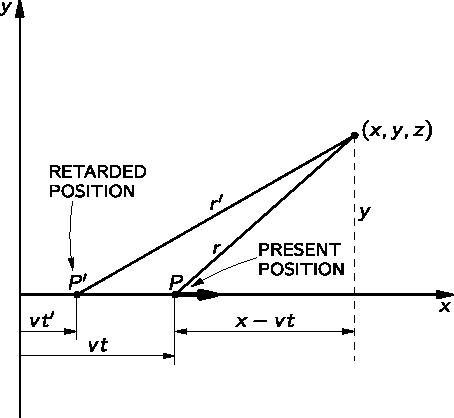
\includegraphics[width=0.7\linewidth]{fyz_fig602.pdf}
      \caption{
               (\cite[s.~707]{Feynman02})}
      \label{fyz_fig602}
    \end{figure}

    \begin{figure}[ht!] %\ref{fyz_fig603}
      \centering
      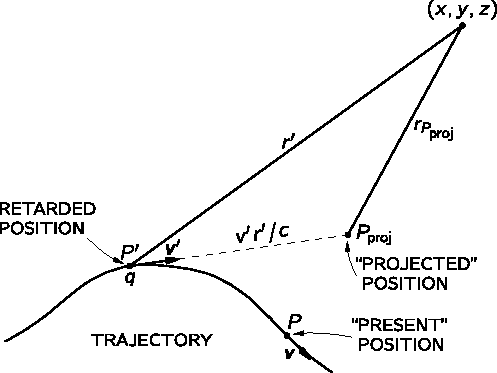
\includegraphics[width=0.7\linewidth]{fyz_fig603.pdf}
      \caption{
               (\cite[s.~707]{Feynman02})}
      \label{fyz_fig603}
    \end{figure}

    \begin{figure}[ht!] %\ref{fyz_fig604}
      \centering
      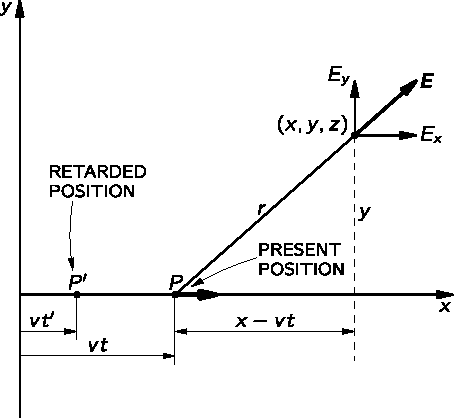
\includegraphics[width=0.7\linewidth]{fyz_fig604.pdf}
      \caption{
               (\cite[s.~707]{Feynman02})}
      \label{fyz_fig604}
    \end{figure}

    \begin{figure}[ht!] %\ref{fyz_fig605}
      \centering
      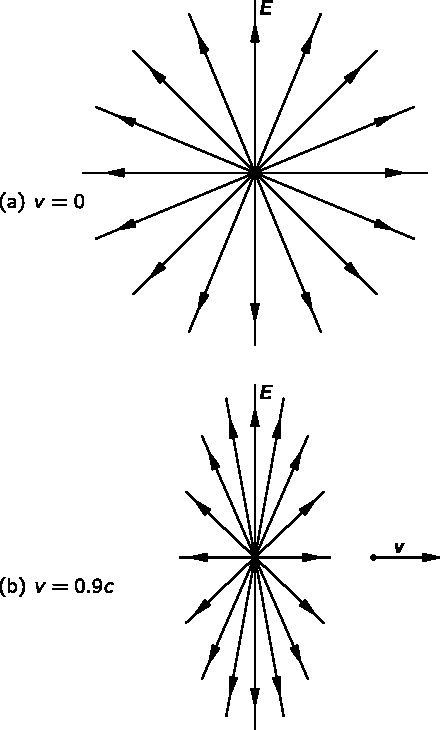
\includegraphics[width=0.7\linewidth]{fyz_fig605.pdf}
      \caption{
               (\cite[s.~707]{Feynman02})}
      \label{fyz_fig605}
    \end{figure}

    \begin{figure}[ht!] %\ref{fyz_fig606}
      \centering
      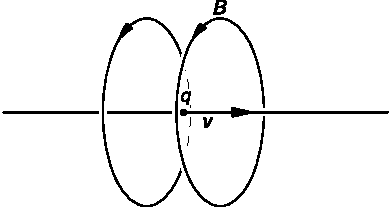
\includegraphics[width=0.7\linewidth]{fyz_fig606.pdf}
      \caption{
               (\cite[s.~707]{Feynman02})}
      \label{fyz_fig606}
    \end{figure}

    \begin{figure}[ht!] %\ref{fyz_fig607}
      \centering
      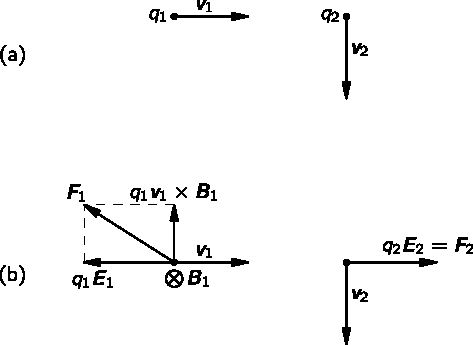
\includegraphics[width=0.7\linewidth]{fyz_fig607.pdf}
      \caption{
               (\cite[s.~707]{Feynman02})}
      \label{fyz_fig607}
    \end{figure}

    \begin{figure}[ht!] %\ref{fyz_fig608}
      \centering
      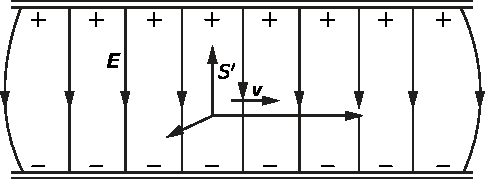
\includegraphics[width=0.7\linewidth]{fyz_fig608.pdf}
      \caption{
               (\cite[s.~707]{Feynman02})}
      \label{fyz_fig608}
    \end{figure}

} %tikzset
%---------------------------------------------------------------------------------------------------
\printbibliography[title={Seznam literatury},heading=subbibliography]
\addcontentsline{toc}{section}{Seznam literatury}